\section{Project Description}

\subsection{Motivation}
Industrialization and climate-change go hand in hand in affecting air quality.
Industrialization worsens climate change and air quality, and climate change
further worsens air quality through natural disasters such as wildfires, acid
rain, or sand storms. It is estimated that 7 million people die from air
pollution globally a year \cite{interplay-climate-change-air-pollution-health}.
Wildfires pose a significant risk for the general population, and especially
those at risk for respiratory infections and people over the age of 65. There is
also a disproportionate increase in air pollution for those in poorer
communities where often times they are close to industrial areas
\cite{socioeconomic-disparities-air-pollution-review}. By providing a low-cost
way of measuring the overall air quality, people can be more educated about the
air quality in their communities, and provide them with the data to back up
their complaints to their local municipalities. For developing countries, they
might be less focused on the environment due to cost constraints, but by
providing a cheap option for measuring air pollution, they can potentially make
more educated decisions about where to make improvements. A low cost air quality
sensor might also be of interest for those that are health conscience, or are
already at risk for respiratory disease, as they can make decisions based on the
current air quality. People living in cities, or other highly industrialized
areas, are also subject to increased air pollution, mostly from motor vehicles
(what create smog and haze), and from factories. Even short term exposure can
cause adverse health affects \cite{health-impacts-air-pollution-review}.
However, the full extent of long term exposure to these pollutants is
inconclusive. What is conclusive is that air pollution is the cause for millions
of deaths world wide each year.

Air quality sensors are very valuable for people living in areas that are high
risk for wildfires, such as California. Smoke from wildfires can be deadly, if
not cause serious health effects depending on the smoke concentration and
exposure time. Based on the air quality, using either the AQI or the AirNow
index, people might need to stay indoors. Another potential use case of an air
quality sensor is the ability to detect wildfire by deploying them to
wildfire-prone areas. By using LoRa, these sensors can provide a wide range of
coverage centered around a LoRa gateway.


\subsection{Goals and Objectives}
\begin{itemize}
    \item The sensor nodes should be low cost.
    \item The sensor nodes should be lightweight.
    \item The sensor nodes should be able to read data from the sensors and transmit that data to a LoRa gateway.
    \item The sensors nodes should be able to communicate over a large enough distance in order to make it feasible to cover large enough area with nodes.
    \item The nodes should require little to no maintenance.
    \item The sensor nodes should be easy to install.
    \item The gateway should be able to connect to the internet to send the data it receives from the nodes to an external server over the internet.
\end{itemize}


\subsection{Requirements Specifications}
In this section, we will describe in detail all of the requirements for our design. However, before going through the entire list, we will first explore three critical requirements. These three requirements will be the ones that we will demonstrate that our finished project satisfies once it has been built. These three requirements can be found in Table \ref{tab:demon-requirements}.

One the first requirements considered for the gateway was total cost. The goal is to keep the cost of the gateway portion of the design to under \$200. Next, a demonstrable requirement specification for this design is its dimensions. Aether’s gateway shall not exceed dimensions greater than 6 x 6 x 6 inches. Given the size and versatility of the sensors that will be used, this should be easily accomplished. Another demonstrable requirement specification the team will focus on is ensuring the gateway does not exceed 5 pounds. This should not be a problem given the fact that most of the components used in the design are extremely compact and lightweight. In regards to communication, each gateway must be capable of supporting a minimum of 8 channels. In addition to this, a gateway must be able to communicate with a node that is located anywhere from 0 to 10 km away from it. These requirements are shown in Table \ref{tab:list-of-requirements}.

For the node requirement specifications, the first thing considered was total cost. It was determined that the node should cost no more than \$150 dollars. It should be cheaper than the gateway design since the node will not have the Lo-Ra-WAN board. Similar to the gateway, the dimensions should not exceed 6 x 6 x 6 inches and the weight should be under 5 pounds, two demonstrable features for the node requirements. Additionally, the nodes should be able to successfully send packets of data to the main server through central Lo-Ra-WAN gateway. Each node will be equipped with a solar panel capable of charging the lithium-ion batteries inside the node, thus giving the nodal system the ability to operate off the grid. The nodes will also be equipped with different power modes to support different demands and efficiently manage battery life. When calculating the AQI level, the nodes must be able to output AQI values in the 300 to 400 range since anything above 300 on an AQI scale is considered hazardous breathing conditions. Node data should be able to be sent to the gateway at a distance up to 10km. Lastly, the node should be able to be configured remotely from the server so field maintenance is kept at a minimum. In Table \ref{tab:list-of-requirements}, we list the node requirement specifications.  


\begin{table}[H]
\centering
\caption{List of requirements}
\begin{tabularx}{\linewidth}{|c|X|}
\hline
No. & Requirement \\
\hline\hline
\rowhl
D.0 & Will be able to dynamically power the node from either the battery, solar panel, or USB \\\hline
\rowhl
D.1 & The node will take sensor measurements and transmit them over LoRaWAN to a server where they be able to be viewed in a graphical and textual format \\\hline
\rowhl
D.2 & The server will send periodic air quality reports and notifications to the
user via Twitter, SMS, and/or email \\\hline
G.0 & The gateway should cost less than \$200 \\\hline
G.1 & The gateway should be no larger than 6 x 6 x 6 inches \\\hline
G.2 & The gateway weight should be no more than than 5 pounds \\\hline
G.3 & The gateway should support at least 8 channels \\\hline
G.4 & The gateway should be able to communicate with nodes up to 10 km away with ideal conditions \\\hline

N.0 & The nodes should cost less than \$150 each \\\hline
N.1 & The nodes should be no larger than 6 x 6 x 6 inches \\\hline
N.2 & The nodes should weigh no more than than 5 pounds \\\hline
N.3 & The nodes should be able to send data packets to the server through a LoRaWAN gateway \\\hline
N.4 & The nodes should each have solar panel(s) to run off the grid indefinitely \\\hline
N.5 & The nodes must support different power usage modes depending on the power budget \\\hline
N.6 & The nodes must be able to calculate the AQI up to at least the 300 to 400 range \\\hline
N.7 & The nodes should be able to send data to a gateway up to 10 km away with ideal conditions \\\hline
N.8 & The nodes should be able to be configured remotely from the server \\\hline

S.0 & The server will host a website to display a map overlaid with air quality data \\\hline
S.1 & The server should be able to send air quality alerts over Twitter and SMS \\\hline
S.2 & The server will be able to automatically register nodes with other supported LoRaWAN Network Servers (Helium, The Things Community, and private networks) \\\hline
\end{tabularx}
\label{tab:list-of-requirements}
\end{table}

On the server side, a host website should be able to display a map overlaid with different air quality data collected from the field. Additionally, the server will have the ability to send air quality reports and alerts via Twitter and SMS. Another requirement specification for the server will be its ability to register nodes with other supported LoRaWAN IoT network servers such as Helium. The server should have the ability to remotely configure nodes in the field to the user's desired operating modes and specifications. The server requirements are listed in Table \ref{tab:list-of-requirements}.


% \begin{table}[H]
% \centering
% \caption{The gateway requirements}
% \begin{tabularx}{\linewidth}{|c|X|c|c|}
% \hline
% No. & Requirement & Value & Units \\
% \hline\hline
% 1.0 & The gateway should cost no more than \$200 & 200 & dollars \\\hline
% 1.1 & The gateway should be no larger than 6" x 6" x 6" & 6x6x6 & inches \\\hline
% 1.2 & The gateway weight should be no more than than 5 pounds & 5 & lbs \\\hline
% 1.3 & The gateway should utilize LoRaWAN with the base station as the gateway with the capacity to connect with up to 8 devices simultaneously. & 8 & nodes \\\hline
% 1.4 & The gateway should be able to communicate with nodes up to 10 km away with ideal conditions & 10	& km \\\hline
% 1.5 & The gateway should be able to communicate with nodes up to 3 km away in an urban environment & 3 & km \\\hline
% 1.6 & The gateway should be able to manage up to 256 nodes & 256 & nodes \\\hline
% \end{tabularx}
% \label{tab:networkingRequirements}
% \end{table}

% \begin{table}[H]
% \centering
% \caption{The sensor node requirements.}
% \begin{tabularx}{\linewidth}{|c|X|c|c|}
% \hline
% No. & Requirement & Value & Units \\
% \hline\hline
% 2.0 & The sensor node should cost no more than \$150 & 150 & dollars \\\hline
% 2.1 & The sensor node should be no larger than 12" x 12" x 12" & 12x12x12 & inches \\\hline
% 2.2 & The sensor node weight should be no more than 10 pounds & 10 & lbs \\\hline
% 2.3 & The sensor node should stay operational without intervention for 1 year & 1 & year \\\hline
% 2.4 & The sensor node sensors should have a maximum tolerance of +/- 20\% & 20 & \% \\\hline
% 2.5 & The sensor node should transmit for no more than 30 seconds every 24 hours & 30 & seconds \\\hline
% \end{tabularx}
% \label{tab:nodeRequirements}
% \end{table}

% \begin{table}[H]
% \centering
% \caption{The gateway and networking engineering specifications}
% \begin{tabularx}{\linewidth}{|c|X|}
% \hline
% No. & Requirement \\
% \hline\hline
% 3.0 & The gateway shall use LoRa and LoRaWAN for the wireless communication protocol \\\hline
% 3.1 & The gateway should adhere to the LoRa Fair Access policy \\\hline
% 3.2 & The gateway should have enough internet bandwidth to support all of its connected nodes \\\hline
% 3.3 & The network shall utilize a star networking topology.\\\hline
% 3.4 & We define a component of our network to be known as a cell, which shall consist of nodes connected to a gateway. \\\hline
% 3.5 & The gateway shall be able communicate with an external server over the internet.\\\hline
% 3.6 & The server shall be hosted on existing web hosting platform.\\\hline
% 3.7 & The server shall host a website that displays data collected from the sensors.\\\hline
% \end{tabularx}
% \label{tab:networkingSpecs}
% \end{table}

% \begin{table}[H]
% \centering
% \caption{The node engineering specifications}
% \begin{tabularx}{\linewidth}{|c|X|}
% \hline
% No. & Requirement \\
% \hline\hline
% 4.0 & The sensor node shall use a radio and antenna that is part of a daughterboard that can be attached to the main PCB.\\\hline
% 4.1 & The node should use a battery and solar panel \\\hline
% 4.2 & The sensor node shall contain a microcontroller. \\\hline
% 4.3 & The sensor node microcontroller shall support the UART protocol.\\\hline
% 4.4 & The sensor node microcontroller shall have at least one ADC.\\\hline
% 4.5 & The sensor node microcontroller shall support JTAG debugging.\\\hline
% 4.6 & The sensor node shall contain a NO2 sensor.\\\hline
% 4.7 & The sensor node shall contain a PM sensor.\\\hline
% 4.8 & The sensor node shall contain a SO2 sensor.\\\hline
% 4.9 & The sensor node shall contain a O3 sensor.\\\hline
% 4.10 & The sensor node shall contain a CO sensor.\\\hline
% \end{tabularx}
% \label{tab:nodeSpecs}
% \end{table}

\begin{table}[H]
\centering
\caption{The constraints.}
\begin{tabularx}{\linewidth}{|X|}

\hline
Constraint \\
\hline\hline
The nodes must be light enough so that they can be affixed to a building or other structure and not be of a concern to fall off \\\hline
The nodes must low cost to be able to placed in greater number \\\hline
The nodes must be able to withstand water from rainfall \\\hline
The nodes must be able to withstand high winds \\\hline
The nodes must be able to withstand temperature extremes \\\hline
The nodes must be able to support a communication range of at least 1 km\\\hline
The nodes must be able to operate on less power than what one solar panel could generate in a single day to allow for operation when there is no sunlight present \\\hline
The gateway must be able to operate off of mains power \\\hline
\end{tabularx}
\label{tab:constraints}
\end{table}

\subsection{House of Quality}
In Figure \ref{fig:hoq}, we provide a comparison between our marketing
parameters and our engineering requirements. The marketing parameters are
qualitative in nature and are chosen based on the qualities that we imagine
customers would be looking for in this product. Accurate means that the sensors
produce a reading that reflects the correct concentration of gases in the air
around the node. It could also refer to having enough nodes to cover an area to
provide a high resolution of sensor data. Low maintenance and reliable are
somewhat related parameters, however, low maintenance refers to the ability of
the node to operate for a long enough period of time without needing to replace
various components and reliable refers to the ability of the node to survive the
outdoor elements and continue to provide quality sensor data over time. Real
time means that the node should be transmitting and reading data from its
sensors as often as possible. Easy to install means that the nodes should be
able to placed in the desired location with minimal effort. Ideally, the nodes
would be able to be placed in wide variety of situations and locations with
relative ease.

In contrast to the marketing parameters, the engineering requirements are
quantitative in nature. Battery life is key since it determines how long the
nodes can be deployed without having to have batteries replaced or recharged.
Node-to-gateway distance refers to how far away a node can be away from a
gateway and is a critical requirement because it directly impacts how large of
and area you can cover with nodes. The number of nodes per gateway is also
important because we would like to minimize the number of gateways required for
any given number of nodes in the network. Sensor accuracy refers specifically to
how far the true measurement of a given gas is from the value outputted by the
sensor. It is given as a $\pm$percentage. Finally, the nodes should of course be
as small, light, and cost as little as possible.

\begin{figure}[H]
    \centering
    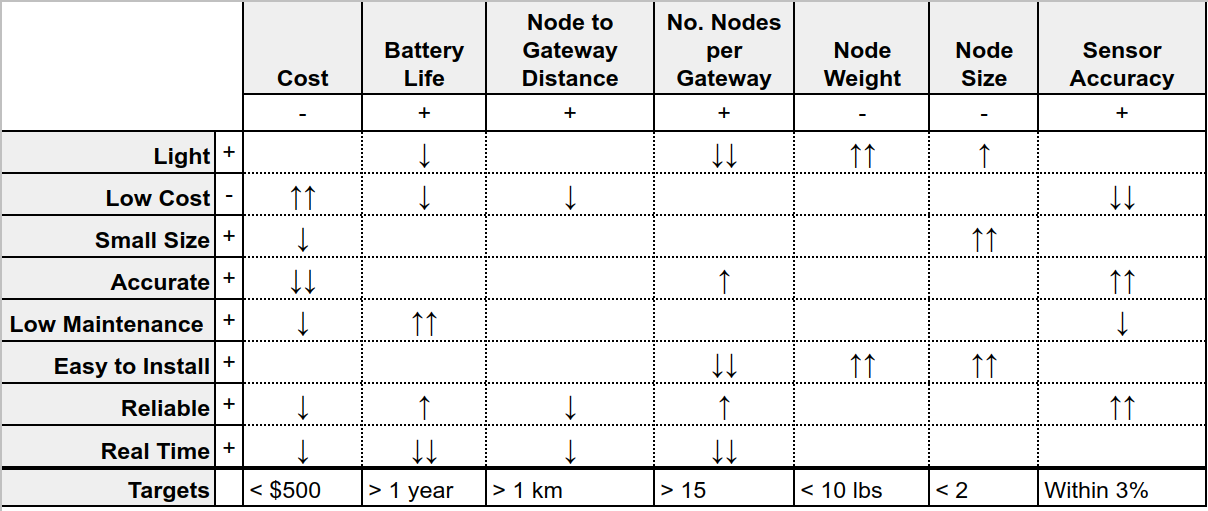
\includegraphics[width=3.5in]{./figures/hoq.png} 
    \caption{The house of quality diagram}
    \label{fig:hoq}
\end{figure}

Almost all of the engineering requirements negatively impact one or more of the
other engineering requirements. Every requirement has a negative impact on the
cost of the nodes and gateways. To increase the battery life, either more
engineering work will be needed to optimize the system (and potentially increase
the BOM) or simply increase the battery capacity. Both of these options increase
the cost.  Likewise, the same is true for the range of the nodes. The range of
the nodes involves finding some way to increase the link-budget. As for the
node's weight and size, these correlate to increased raw material costs and/or
increased manufacturing costs, especially for the node size. Lastly, sensor
accuracy affects the cost because of the engineering, material costs, and
manufacturing needed to create more accurate sensors. Battery life also heavily
negatively affects range, because of the need for active RF circuitry,
namely amplification, when transmitting data. The size of the nodes helps battery
life since it allows for a battery with a higher capacity. It also helps the
range of the nodes by allowing for a larger antenna, which helps with increasing
the receive sensitivity. Lastly, the weight and size of the nodes negatively
impact each other since, because usually the larger the node is the more it is
going to weigh.

\subsection{Block Diagrams}
In this section, we show the block diagrams for different parts of our design. Our block diagrams also indicate who is going to be responsible for each part of the design. We also indicate the current status of each block in the diagram. These statuses include RES, meaning that this portion of the design is currently being investigated, and TBA, meaning that this portion of the design will be purchased outright. The sensor node is our primary design focus for this project. The block diagram for the sensor node shows how the various sensors will interface with the selected system controller as well as how we plan to power the system via a battery and a solar panel. The interface between the system controller and the LoRa module is also shown. This block diagram can be found in Figure \ref{fig:hwNodeBD}. In addition, a more detailed description of each block in the diagram can found in Table \ref{tab:Node_Hardware_BD_Description}.

% Block Diagram for Node HW
\begin{figure}[H]
    \centering
    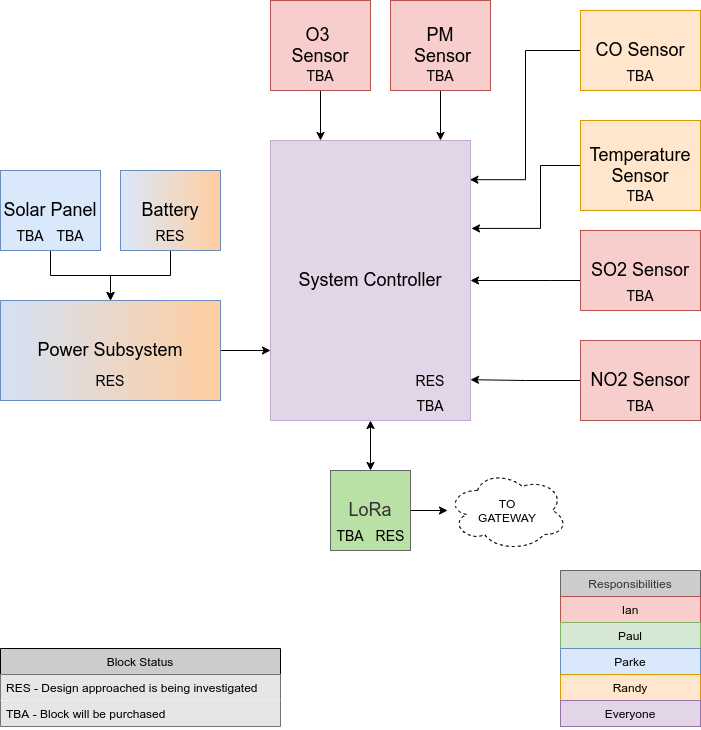
\includegraphics[width=5.3in]{"./figures/hwNodeBD.png"} 
    \caption{The block diagram for the sensor node hardware.}
    \label{fig:hwNodeBD}
\end{figure}

Another key component of our design is the LoRaWAN gateway. We do not plan on entirely designing the gateway. However, we did create a block diagram demonstrating how we we would plan to set up a gateway using off-the-shelf components. The block diagram for the gateway shows how a selected LoRa module would interface with a development board. This development board would need to be able to support connecting with a LoRa module. This development board would also need to be able to interface with an Ethernet port. Ethernet is essential for the gateway to be able to connect to the internet. The block diagram also shows how we plan to simply connect the gateway to mains power. It is unnecessary for the gateway to be powered via battery. This will make worrying about power consumption less of a design constraint for the gateway. This block diagram can be found in Figure \ref{fig:hwBaseStationBD}. In addition, a more detailed description of each block in the diagram can found in Table \ref{tab:descHWBaseStationBD}.

% Block Diagram for gateway HW
\begin{figure}[H]
    \centering
    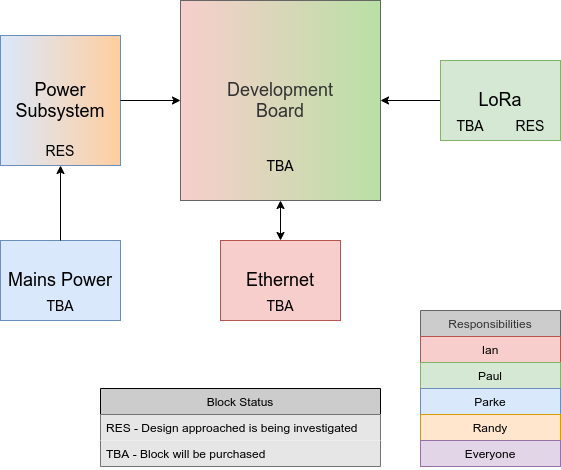
\includegraphics[width=5.3in]{"./figures/hwGatewayBD.png"} 
    \caption{The block diagram for the gateway hardware.}
    \label{fig:hwBaseStationBD}
\end{figure}

\begin{figure}[H]
    \centering
    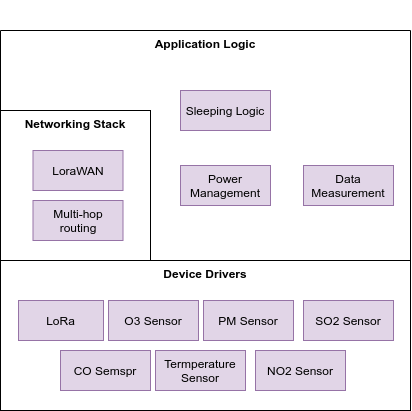
\includegraphics[width=4in]{"./figures/swNodeBD.png"} 
    \caption{The block diagram for the node software.}
    \label{fig:swNodeBD}
\end{figure}
\begin{table}[H]
    \centering
    \caption{A description of each block in the sensor node hardware block diagram.}
    \begin{tabularx}{\linewidth}{|c|X|}
        \hline
        Block Name & Description \\ 
        \hline
        Battery & The battery will take in power from the power subsystem and will store whatever is left over from the consumption by the system controller. \\\hline
        Power Subsystem & The power subsystem will take in and regulate power from the solar panel charging the battery as well as taking power from the battery for whatever needs the system controller requires. The power subsystem will also invert the DC power from the solar panel and battery to AC if required. \\\hline
        Solar Panel & The solar panel will feed power to the power subsystem where a solar power controller will be placed to take in the generated power. \\\hline
        System Controller & The system controller take in and process data from the sensors and output data to the LoRa transceiver. \\\hline
        Temperature Sensor & The temperature sensor will take a measurement of the current temperature and send it to the system controller. \\\hline
        O$_3$ Sensor & The temperature sensor will take a measurement of the current amount of detected ozone (O$_3$) and send it to the system controller. \\\hline
        CO Sensor & The temperature sensor will take a measurement of the current amount of detected carbon monoxide (CO) and send it to the system controller. \\\hline
        SO$_2$ Sensor & The temperature sensor will take a measurement of the current amount of detected sulfur dioxide (SO$_2$) and send it to the system controller. \\\hline
        NO$_2$ Sensor & The temperature sensor will take a measurement of the current amount of detected nitrogen dioxide (NO$_2$) and send it to the system controller. \\\hline
        PM Sensor & The temperature sensor will take a measurement of the current amount of detected particulate matter (PM) and send it to the system controller. \\\hline
        LoRa & The LoRa transceiver will receive data from the system controller and send that data to the gateway. \\\hline
    \end{tabularx}
    
    \label{tab:Node_Hardware_BD_Description}
\end{table}
\begin{table}[H]
    \centering
    \caption{A description of each block in the gateway hardware block diagram.}
    \begin{tabularx}{\linewidth}{|c|X|}
        \hline
        Block Name & Description \\ 
        \hline\hline
        Power Subsystem & The power subsystem will take in power from the battery for whatever needs the development board requires. The power subsystem will also invert the DC power from the solar panel and battery to AC if required. \\\hline
        Mains Power & This is the AC power coming from a wall outlet. \\\hline
        Ethernet & The Ethernet module will allow the development board to connect to the internet. \\\hline
        LoRa & The LoRa transceiver will receive data from the sensor nodes and send that data to the development board. \\\hline
        Development Board & The development board will process the sensor data received from the sensor nodes. This data will then be sent to an external server over the internet where it can be analyzed. \\\hline
    \end{tabularx}
    \label{tab:descHWBaseStationBD}
\end{table}
\begin{table}[H]
    \centering
    \caption{A description of each block in the sensor node software block diagram.}
    \begin{tabularx}{\linewidth}{|c|X|}
        \hline
        Block Name & Description \\ 
        \hline
        Power Management & This software will responsible for controlling and monitoring the power subsystem.  \\\hline
        Data Management & This software will be responsible for processing data received from the sensors. \\\hline
        Sleeping Logic & This software will handle the logic for switching between taking sensor measurements and residing in a low-power "sleep" mode between sensor measurements. \\\hline
        LoRa & This is a device driver for the LoRa transceiver. \\\hline
        Temperature Sensor & This is a device driver for the temperature sensor. \\\hline
        O$_3$ Sensor & This is a device driver for the O$_3$ sensor. \\\hline
        CO Sensor & This is a device driver for the CO sensor. \\\hline
        SO$_2$ Sensor & This is a device driver for the SO$_2$ sensor. \\\hline
        NO$_2$ Sensor & This is a device driver for the NO$_2$ sensor. \\\hline
        PM Sensor Sensor & This is a device driver for the PM sensor. \\\hline
        LoRaWAN & This handles the networking for the LoRa networking. \\\hline
        Multi-hop Routing & This software will control how traffic is routed around the sensor node network. \\\hline
    \end{tabularx}
    \label{tab:descSWNodeBD}
\end{table}
